\section{賭け金の概念の導入}
ここまで勝率により評価をしてきた。しかしプレイヤーの最終目標はゲームに勝つことではなく利得を増やすことである。
ブラックジャックにはダブルダウンやスプリットがあるので勝率が低くても利得を増やす手段がある。
また、賭け額を操作することで利得を増やすことができる。例えば、10戦して1勝9敗だとしても1勝の時にだけ
多額を賭けていれば勝率が低くても高い利得を得ることができる。なのでここからは賭け金を導入して検証を行う。
方法として用いる戦略によって所持金がどのように推移するのかを調査する。
比較対象となる戦略は次の通りである。

\begin{itemize}
  \item BS:ダブルダウン・スプリットを含むベーシックストラテジー
  \item BS_HS:ヒット・スタンドのみで構成されたベーシックストラテジー
  \item GA戦略:遺伝的アルゴリスムを用いて導出された戦略

\end{itemize}

以上の3つの戦略について、これから詳細に説明する。
\bunseki{※轟木文弥}

\subsection{BS}
ベーシックストラテジーはブラックジャックにおける有効な戦略の一つである。
表\ref{bs_hard}、表\ref{bs_soft}、表\ref{bs_sprit}に示すように、ダブルダウンやスプリットがあるため表の複雑性が高いという特徴がある。
\bunseki{※轟木文弥}

\begin{table}[htbp]
  \centering
  \caption{BSのハードハンド\label{bs_hard}}
  \begin{tabular}{|c|c|c|c|c|c|c|c|c|c|c|c|}
    \hline
    \multicolumn{2}{|c|}{} & \multicolumn{10}{|c|}{ディーラーのアップカード} \\ \hline
    \multicolumn{2}{|c|}{} & 2 & 3 & 4 & 5 & 6 & 7 & 8 & 9 & 10 & A \\ \hline
    手札 & 8以下 & H & H & H & H & H & H & H & H & H & H \\ \cline{3-12}
              & 9 & H & D & D & D & D & H & H & H & H & H \\ \cline{3-12}
              & 10 & D & D & D & D & D & D & D & D & H & H \\ \cline{3-12}
              & 11 & D & D & D & D & D & D & D & D & D & D \\ \cline{3-12}
              & 12 & H & H & S & S & S & H & H & H & H & H \\ \cline{3-12}
              & 13~16 & S & S & S & S & S & H & H & H & H & H \\ \cline{3-12}
              & 17以上 & S & S & S & S & S & S & S & S & S & S \\ \hline
  \end{tabular}
\end{table}

\begin{table}[htbp]
  \centering
  \caption{BSのソフトハンド\label{bs_soft}}
  \begin{tabular}{|c|c|c|c|c|c|c|c|c|c|c|c|}
    \hline
    \multicolumn{2}{|c|}{} & \multicolumn{10}{|c|}{ディーラーのアップカード} \\ \hline
    \multicolumn{2}{|c|}{} & 2 & 3 & 4 & 5 & 6 & 7 & 8 & 9 & 10 & A \\ \hline
    手札 & A2 & H & H & H & H & D & H & H & H & H & H \\ \cline{3-12}
              & A3 & H & H & H & H & D & H & H & H & H & H \\ \cline{3-12}
              & A4 & H & H & D & D & D & H & H & H & H & H \\ \cline{3-12}
              & A5 & H & H & D & D & D & H & H & H & H & H \\ \cline{3-12}
              & A6 & H & D & D & D & D & H & H & H & H & H \\ \cline{3-12}
              & A7 & D & D & D & D & D & S & S & H & H & S \\ \cline{3-12}
              & A8 & S & S & S & S & D & S & S & S & S & S \\ \cline{3-12}
              & A9 & S & S & S & S & S & S & S & S & S & S \\ \cline{3-12}
              & A10 & S & S & S & S & S & S & S & S & S & S \\ \hline
  \end{tabular}
\end{table}

\begin{table}[htbp]
  \centering
  \caption{BSのスプリット\label{bs_sprit}}
  \begin{tabular}{|c|c|c|c|c|c|c|c|c|c|c|c|}
    \hline
    \multicolumn{2}{|c|}{} & \multicolumn{10}{|c|}{ディーラーのアップカード} \\ \hline
    \multicolumn{2}{|c|}{} & 2 & 3 & 4 & 5 & 6 & 7 & 8 & 9 & 10 & A \\ \hline
    手札 & AA & P & P & P & P & P & P & P & P & P & P \\ \cline{3-12}
              & 22 & H & H & P & P & P & P & H & H & H & H \\ \cline{3-12}
              & 33 & P & P & P & P & P & P & H & H & H & H \\ \cline{3-12}
              & 44 & H & H & D & P & P & H & H & H & H & H \\ \cline{3-12}
              & 55 & D & D & D & D & D & D & D & D & H & H \\ \cline{3-12}
              & 66 & P & P & P & P & P & H & H & H & H & H \\ \cline{3-12}
              & 77 & P & P & P & P & P & P & H & H & H & H \\ \cline{3-12}
              & 88 & P & P & P & P & P & P & P & P & P & P \\ \cline{3-12}
              & 99 & P & P & P & P & P & S & P & P & S & S \\ \cline{3-12}
              & 1010 & S & S & S & S & S & S & S & S & S & S \\ \hline
  \end{tabular}
\end{table}

\subsection{BS_HS}
BSの複雑性が高いという問題を解決するために、BSをヒットとスタンドのみで構成した。
スプリットは使用せずにハードハンドとして処理した。また、ダブルダウンは基本的にヒットとしたが、ソフトハンドのA7、A8の行はスタンドとした。
表\ref{bs_hs_hard}、表\ref{bs_hs_soft}}に示すように、ダブルダウンとスプリットがなくなったことで複雑性が低くなっている。
\bunseki{※轟木文弥}

\begin{table}[htbp]
  \centering
  \caption{BS_HSのハードハンド\label{bs_hs_hard}}
  \begin{tabular}{|c|c|c|c|c|c|c|c|c|c|c|c|}
    \hline
    \multicolumn{2}{|c|}{} & \multicolumn{10}{|c|}{ディーラーのアップカード} \\ \hline
    \multicolumn{2}{|c|}{} & 2 & 3 & 4 & 5 & 6 & 7 & 8 & 9 & 10 & A \\ \hline
    手札 & 11以下 & H & H & H & H & H & H & H & H & H & H \\ \cline{3-12}
              & 12 & H & H & S & S & S & H & H & H & H & H \\ \cline{3-12}
              & 13~16 & S & S & S & S & S & H & H & H & H & H \\ \cline{3-12}
              & 17以上 & S & S & S & S & S & S & S & S & S & S \\ \hline

\begin{table}[htbp]
  \centering
  \caption{BS_HSのソフトハンド\label{bs_hs_soft}}
  \begin{tabular}{|c|c|c|c|c|c|c|c|c|c|c|c|}
    \hline
    \multicolumn{2}{|c|}{} & \multicolumn{10}{|c|}{ディーラーのアップカード} \\ \hline
    \multicolumn{2}{|c|}{} & 2 & 3 & 4 & 5 & 6 & 7 & 8 & 9 & 10 & A \\ \hline
    手札 & A2~A6 & H & H & H & H & H & H & H & H & H & H \\ \cline{3-12}
              & A7 & S & S & S & S & S & S & S & H & H & H \\ \cline{3-12}
              & A8~A10 & S & S & S & S & S & S & S & S & S & S \\ \cline{3-12}
              & AA & H & H & H & H & H & H & H & H & H & H \\ \hline

\subsection{GA戦略}
遺伝的アルゴリズムを用いて導出した。
表\ref{ga_hard}、表\ref{ga_soft}}に示すように、HとSのみで構成され複雑性が低くなっている。

\begin{table}[htbp]
  \centering
  \caption{GA戦略のハードハンド\label{ga_hard}}
  \begin{tabular}{|c|c|c|c|c|c|c|c|c|c|c|c|}
    \hline
    \multicolumn{2}{|c|}{} & \multicolumn{10}{|c|}{ディーラーのアップカード} \\ \hline
    \multicolumn{2}{|c|}{} & 2 & 3 & 4 & 5 & 6 & 7 & 8 & 9 & 10 & A \\ \hline
    手札 & 13以下 & H & H & H & H & H & H & H & H & H & H \\ \cline{3-12}
              & 14以上 & S & S & S & S & S & S & S & S & S & S \\ \hline

\begin{table}[htbp]
  \centering
  \caption{GA戦略のソフトハンド\label{ga_soft}}
  \begin{tabular}{|c|c|c|c|c|c|c|c|c|c|c|c|}
    \hline
    \multicolumn{2}{|c|}{} & \multicolumn{10}{|c|}{ディーラーのアップカード} \\ \hline
    \multicolumn{2}{|c|}{} & 2 & 3 & 4 & 5 & 6 & 7 & 8 & 9 & 10 & A \\ \hline
    手札 & AA~A6 & H & H & H & H & H & H & H & H & H & H \\ \cline{3-12}
              & A7 & S & S & S & S & S & S & S & S & H & H \\ \cline{3-12}
              & A8~A10 & S & S & S & S & S & S & S & S & S & S \\ \hline




\subsection{一定ベット}
複数の戦略で常に一定額をベットした場合の所持金推移を調べ比較した。
シミュレーションの条件は次のように設定した。
デック数は6、プレイヤーは1人でディーラーとプレイヤーの1対1、初期所持金は1000で
毎回10ずつ賭けた。
試行回数は40ゲームを1セットとして、それを50000セット行った。
シミュレーションの結果を図\ref{bet-defineite}と表\ref{table:data_type}に示す。
\bunseki{※轟木文弥}

\begin{figure}[h]
 \begin{tabular}{cc}
 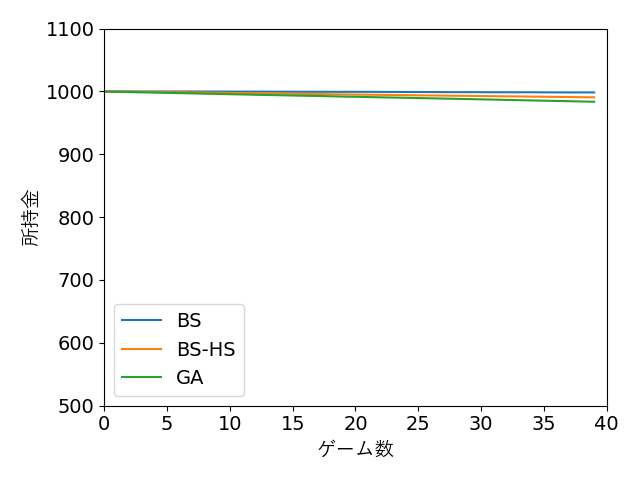
\includegraphics{./figure/bet-defineite-ver5.png}
 \caption{一定ベットの結果}
\label{bet-defineite-figure}
\end{tabular}
\end{figure}

\begin{table}[H]
 \caption{一定ベットでの所持金}
\label{bet-defineite-table}
 \begin{center}
  \begin{tabular}{|c|c|c|}
    \hline 
    \multicolumn{40回目の平均所持金} & \multicolumn{標準偏差} \\
    \hline BS & 998.328 & 73.538  \\
    \hline BS_HS &990.499 & 62.013  \\
    \hline GA戦略 & 983.470 & 62.401  \\
    \hline
  \end{tabular}
 \end{center}
\end{table}

今回は一定額を賭けてシミュレーションした。その結果を図\ref{bet-defineite}と表\ref{table:data_type}にまとめた。図\ref{bet-defineite}を見ると全ての戦略が右肩下がり
になっていることがわかる。また、どの戦略でも初期所持金の1000を超えることがなかった。
ここから賭け額を変化させることで良い結果になる可能性があると考えた。
\bunseki{※轟木文弥}

\section{カウンティングの概念の導入}
賭け額を戦略的に変化させる手法として、既存の戦略であるカウンティングという手法を
用いる。カウンティングとは、使用されたカードを覚えておくことで残りのデックの中身を推測
し、有利不利に合わせて賭け額を操作するという手法である。しかし、使用された
カードを全て覚えるというのは難易度が高く、実際には不可能である。なので簡易化のために
使用されたカードの種類に応じてカウントを増減させ、そのカウントによってプレイヤーの
有利不利を判断するというのが一般的である。プレイヤーが有利な時は賭け額を増やし、
不利な時は賭け額を減らす。
\bunseki{※轟木文弥}
